
\subsection{Creating a new CaesarJ project}
From the File menu select new... . If "Caesar Project" appears
in the list, select it.\\\\
If it doesn't, this is probably the first time you've used the plugin - select "Other" and then "Caesar" and "Caesar Project".
\begin{figure}[htbp]
	\centering
		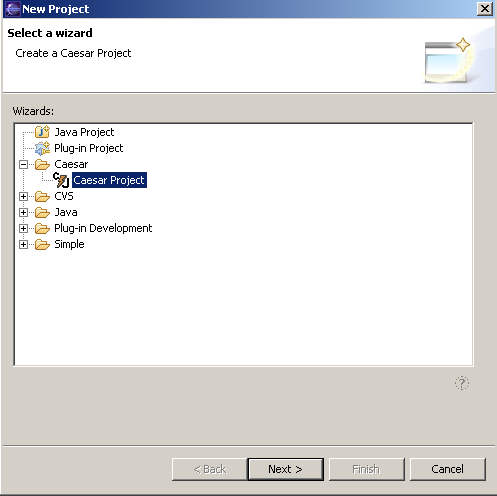
\includegraphics[width=0.85\textwidth]{images/project_wizard.png}
	\label{fig:project_wizard}
\end{figure}\newpage

The new project wizard appears:
\begin{figure}[htbp]
	\centering
		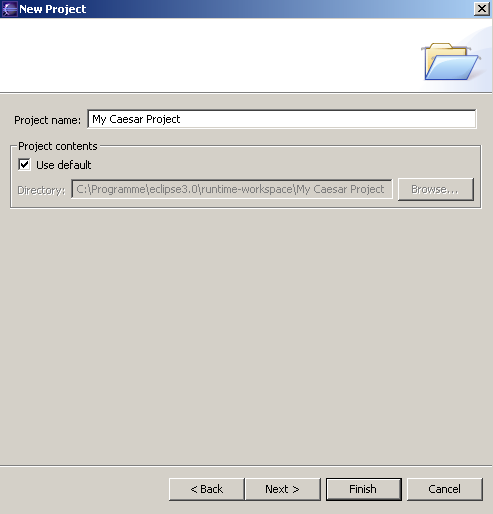
\includegraphics[width=0.45\textwidth]{images/project_wizard2.png}
	\label{fig:project_wizard2}
\end{figure}

This wizard has identical behaviour to the new Java project wizard (except of course that
it creates a project with the Caesar nature).\\
When you click "Finish" on the new project wizard, your project will be created.\\\\
Now you propperly want to open the "Caesar Perspective". Select Window -$>$ Open Perspective -$>$ Others -$>$ CaesarJDT Perspective.
If this is the first time you've used CJDTP, you will see the following dialog pop-up:\\
\begin{figure}[htbp]
	\centering
		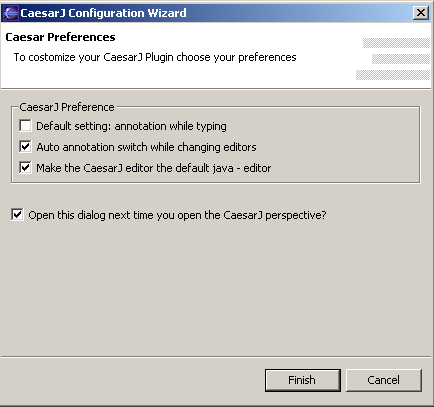
\includegraphics[width=0.5\textwidth]{images/view_properties.png}
	\label{fig:view_properties}
\end{figure}


This dialog configures some Eclipse settings that will make your life much easier when
working with CaesarJ projects. Leave everything selected and click
"Finish".
